\documentclass{beamer}
\usetheme{PaloAlto}
\usecolortheme{albatross}
\usepackage{etoolbox}

\definecolor{Antra}{RGB}{105,105,105}
\definecolor{AntraB}{RGB}{105,105,125}
\definecolor{Gris}{RGB}{80,80,85}
\setbeamercolor*{structure}{fg=Antra!50,bg=AntraB}

\setbeamercolor*{palette primary}{use=structure,fg=white,bg=Gris}
\setbeamercolor*{palette secondary}{use=structure,fg=white,bg=Gris}


\setbeamercolor*{background canvas}{bg=Antra,fg=Antra}

\setbeamercolor*{normal text}{bg=AntraB,fg=Antra!10}
\setbeamercolor*{navigation symbols}{bg=AntraB,fg=Antra!10}

\setbeamertemplate{sidebar right}

\beamertemplatenavigationsymbolsempty


\title[Revue de projet Final]{Projet Aéroglisseur \\Revue de Projet Finale}
\author[]{Florian POUTHIER - Tristan DRUSSEL}
\date{Mai 2020}
\institute{4ème année Génie Électrique - INSA Strasbourg}
\setbeamertemplate{footline}
{
\leavevmode% 
 \begin{beamercolorbox}[wd=0.3333\paperwidth,center,ht=0.025\paperheight,dp=0.0125\paperheight]{Gris}
   \hspace*{2em}\insertshortauthor\hspace*{2em}
 \end{beamercolorbox}
  \begin{beamercolorbox}[wd=0.3333\paperwidth,center,ht=0.025\paperheight,dp=0.0125\paperheight]{Gris}
 \hspace*{2em}  \insertframenumber\hspace*{2em}
 \end{beamercolorbox}
  \begin{beamercolorbox}[wd=0.3333\paperwidth,right,ht=0.025\paperheight,dp=0.0125\paperheight]{Gris}
  \hspace*{2em} \insertdate\hspace*{2em}
 \end{beamercolorbox}
  \vskip0pt
}


\begin{document}
	\begin{frame}[noframenumbering,plain]
		\titlepage
	\end{frame}
	\begin{frame}
		\frametitle{Aperçu}
	%Contexte du projet
	%organisation du travail,problématique, questionnement reformulation du rpbleme
		\begin{columns}[T]
	  		\begin{column}{0.5\textwidth}
	    	Réalisation d'un aéroglisseur sur la base du Chticat\\
	    	Mise en oeuvre de l'électronique de puissance, de l'électronique numérique et de la mécanique
	  		\end{column}
	  		\begin{column}{0.5\textwidth}
	    	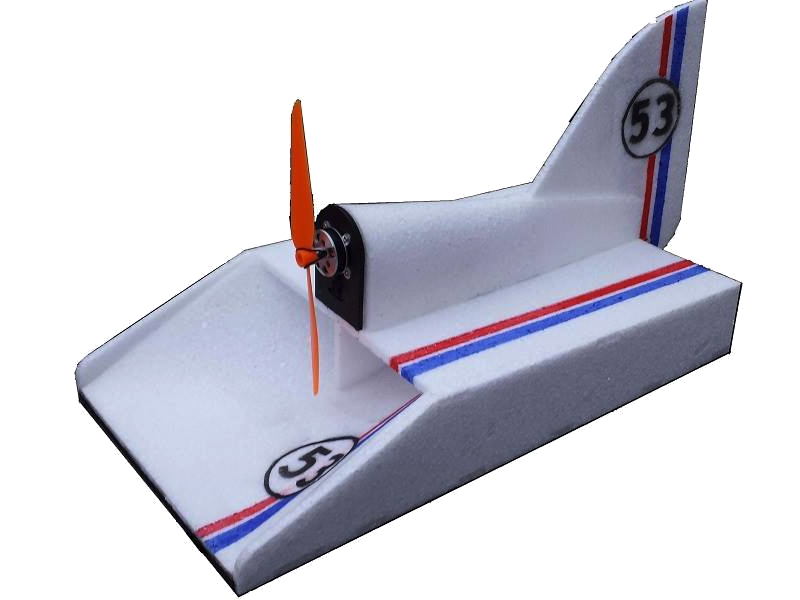
\includegraphics[width=\textwidth]{"../Illus/Chticat.png"}
	  		\end{column}
		\end{columns}
	\end{frame}
	\begin{frame}
	%Plan d'intervention succinct
		\frametitle{Sommaire}
		\tableofcontents
	\end{frame}
	\begin{frame}{L'aspect mécanique}
		\section[Mécanique]{L'aspect Mécanique}
		\begin{columns}[T]
	  		\begin{column}{0.5\textwidth}
	    	\begin{itemize}
	    		\item Récupération des sources
	    		\item Adaptation du modèle
	    	\end{itemize}
	  		\end{column}
	  		\begin{column}{0.5\textwidth}
	    	\includegraphics[width=\textwidth]{"../Illus/3Dview.png"}
	  		\end{column}
		\end{columns}
		
	\end{frame}
	\begin{frame}{Électronique Numérique}
		\section[ENUM]{L'aspect Électronique Numérique}
		
	\end{frame}
	\begin{frame}{Électronique Numérique:Communication Bluetooth}
		\subsection[Bluetooth]{Communication Bluetooth}
	
	\end{frame}
	\begin{frame}
		\section[ENPU]{L'aspect Électronique de Puissance}
		
		
	\end{frame}
	\begin{frame}
		\section[Poursuites]{Poursuites du projet}
		\frametitle{}
		\insertframenumber/\inserttotalframenumber
	\end{frame}
	
	\begin{frame}
	\section*{Conclusion}
	\frametitle{Conclusion}
	%Conclusion
	\insertframenumber/\inserttotalframenumber
	\end{frame}
	\begin{frame}
	\section*{}
		%remerciement
		\frametitle{Merci de votre attention}
		\titlepage
	\end{frame}
\end{document}